\documentclass[main.tex]{subfiles}
\begin{document}

\section{Non-parametric Spectrum Estimation}

In the world of signal processing, the ability to process and analyse the signal in the frequency domain is essential. Unlike on paper, real signals do not span \textit{ad infinitum}, are limited and often windowed. Calculating the fourier transform becomes impossible, and other spectral estimation methods must be applied. 

Non-parametric spectral estimation applies a fourier-like transform (the DFT) to a real world signal. Non-parametric spectral estimation is perfect when analysing a general set of signals, as few assumptions on the underling signals are made.

In this first section, the basics of spectral estimation with focus on non-parametric estimation are investigated.


\subsection{Discrete Fourier Transform Basis}

The Discrete Fourier Transform is a modification of the Fourier Transform that can be applied to discrete time signals, and is defined as 

\begin{equation}
X(w) = \sum_{n=-\infty}^{\infty} x(n)e^{jwn}
\end{equation}

\subsubsection{Ideal Fourier Spectrum and DTFT}

Before diving into estimations with matlab, it's useful to be able to sketch out the expected results for the ideal Fourier specturm, as well as the DFT for a signal, and to compare this with the restuls we will gather in Matlab. To this purpose, a 20Hz signal is considered, and it's fourier spectrum is drawn side by side with the DFT (\textit{Using a windowed input}).


\begin{figure}[H]
	\centering
	\begin{subfigure}[b]{\textwidth}
		\centering
		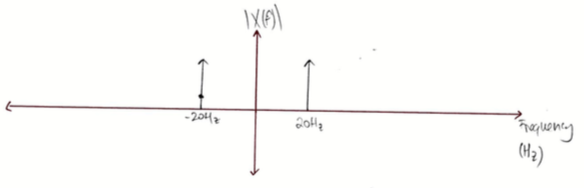
\includegraphics[width=0.8\textwidth]{images/1-1-a-2.png}
		\caption{Ideal tranform of a single 20Hz wave with no noise}
		\label{fig:1-1-a-1}
	\end{subfigure}%
	
	\begin{subfigure}[b]{\textwidth}
		\centering
		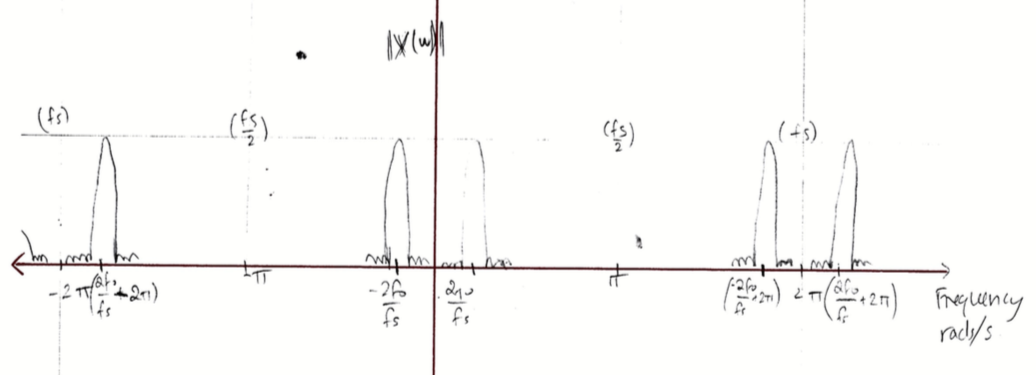
\includegraphics[width=0.8\textwidth]{images/1-1-a.png}
		\caption{DFT transform of 20Hz signal passed through a generic window. Note the signal is repeated at $2\pi$. }
		\label{fig:1-1-a-2}
	\end{subfigure}%
\end{figure}

It's important to note that the DFT will be symmetrical around the y-axis, and will be repeated every $2\pi$. \textit{Sampling in the time domain is repitition on the frequency domain. Sampling in the frequency domain is repitition in the time domain}.


\subsubsection{Comparison to Matlab result}

Turning to matlab, the results found above can be verified. By using the DFT with two different point-numbers, the two results found above are plotted.

\begin{figure}[H]
	\centering 
	\resizebox{0.8\textwidth}{!}{\input{matlabimages/1-1-b.tikz}}
	\caption{100 (left) and 1000 (right) point DFT results using matlab's {\tt fft} function. The {\tt fftshit} function has been used to center the results around the y-axis.}
	\label{fig:q1_1_b}
\end{figure}

Figure~\ref{fig:q1_1_b} clearly shows the effect of windowing on an otherwise perfect sinusoid. The left image shows two clean peaks at $20$ and $-20$ Hz, as expected. When increasing the FFT size for the same signal of 100 samples, the original signal is zero padded to the right to match the fft-size. Therefore, when taking a 1000-point FFT, the sinusoid is zero padded with 900 zeros. Conceptually, this is the same effect of the infinite sinuoid being windowed by a rectangular window over the first 100 samples.

\paragraph{As the input for the 1000-point FFT is windowed,} a number of lobes appear in the frequency spectra. This comes from two fact; 
\begin{enumerate}
	\item $rect(t) \Leftrightarrow sinc(\pi f)$, which will generate a main lobe and a number of side lobes when looking at the magnitude spectrum.
	\item Multiplication in the time domain is convolution in the frequency domain, therefore a sinc will appear centered at $\pm 20Hz$ when looking at the magnitude spectrum.
\end{enumerate}

It's imporant to note that the {\tt fft} function will only give a result over a single spectrum of $[-\pi,\pi)$ (or $[0, 2\pi)$ without {\tt fftshift}). However, the true DFT will be repeated every multiple of $2\pi$, such that $X(w) = X(w+2\pi)$.

\subsubsection{Incoherent Sampling}

Zero padding as in 1.1(b) is not the only scenario where the DFT of a single frequency wave turns into a fuller spectrum. Any discontinuity in the time domain will also result in lobes, rather than diract functions in the frequency response (\textit{for clean sinusoids}). This has the same effect as the windowing seen above. 

\paragraph{Discontinuous signals} will display similar properties as zero-padded signals (see figure \ref{fig:q1_1_b}). To overcome this, careful consideration of the time chunk passed through the FFT should be made. In reality, this is rarely possible, so a range of other windows (Hamming, Hanning, Bartlett) are considered to smoothen out discontinuities. These are discussed in detail futher in this section.

\paragraph{Frequency Resolution.} In addition to the discontinuity, which will explain why a full spectrum rather than two diract functions are seen in figure~\ref{fig:q1_1_c}, taking the FFT over 100 points makes it hard to see the peak of the central lobe. As the FFT with N points will have a frequency resolution of $f_s/N$, in the case where $N=100$, the resolution is 10Hz. Therefore, at $24Hz$ where a dirac is expected, there is no sample.

\paragraph{It is therefore important to ensure the fft size} gives the most appropriate frequency resolution required in each case. There is generally a tradeoff between the computational complexity of increasing the FFT size and the resulting frequency resolution.

\begin{figure}[H]
	\centering 
	\resizebox{0.7\textwidth}{!}{\input{matlabimages/1-1-c.tikz}}
	\caption{100 point DFT of a 24Hz wave}
	\label{fig:q1_1_c}
\end{figure}


\paragraph{To solve the incoherent sampling problem,} the FFT window should be increased to improve the frequency resolution.




















\subsection{Properties of Power Spectral Density (PSD)}

Starting from the two equations of the PSD,

\begin{align}
P(\omega) &= \sum_{k=-\infty}^{\infty}r(k)e^{-jwk}\\
&= \lim_{N \rightarrow \infty} 
E \left[ 
		\frac{1}{N} \left| \sum_{n=0}^{N-1}x(n)e^{-jnw} \right| ^2
\right] \label{eq:1-0-psd-1}
\end{align}

As the sum in equation~\ref{eq:1-0-psd-1} is a complex number, it can be replaced by a conjugate multiplication

\begin{align}
P(\omega) &= \lim_{N \rightarrow \infty} 
E \left[ 
\frac{1}{N} \left(\sum_{n=0}^{N-1}x(n)e^{-jnw}\sum_{m=0}^{N-1}x^*(n)e^{jmw}\right)
\right]\\
&= \lim_{N \rightarrow \infty} 
E \left[ 
\frac{1}{N} \sum_{n=0}^{N-1} \sum_{m=0}^{N-1} \left(x(n)x^*(m)e^{-j(n-m)w}\right)
\right]\\
&= \lim_{N \rightarrow \infty} 
\frac{1}{N} \sum_{n=0}^{N-1} \sum_{m=0}^{N-1} E \left[ x(n)x^*(m)
\right] e^{-j(n-m)w} \label{eq:1-0-psdtwosum} \\
\end{align}

Using the auto-correlation function for a function $x(n)$

\begin{align}
r_{xx}(k) &= E\left[x(n)x^*(n-k)\right]\\
r_{xx}(n-k) &= E\left[x(n)x^*(k)\right]
\end{align}

Therefore, eq~\ref{eq:1-0-psdtwosum} can be re-written as a function of the auto correlation function,

\begin{align}
P(\omega) &= \lim_{N \rightarrow \infty} 
\frac{1}{N} \sum_{n=0}^{N-1} \sum_{m=0}^{N-1} r_{xx}(n-m) e^{-j(n-m)w}  \\
\end{align}

These two sums can be combined into a single sum by considering the number of times each combination of m and n happens for the ACF. %TODO explain this better

\begin{align}
P(\omega) &= \lim_{N \rightarrow \infty} 
\frac{1}{N} \sum_{n=0}^{N-1} \sum_{m=0}^{N-1} r_{xx}(n-m) e^{-j(n-m)w}\\
&= \lim_{N \rightarrow \infty} 
\frac{1}{N} \sum_{\tau=-(N-1)}^{N-1} \left(1-\frac{|\tau|}{N}\right) r_{xx}(\tau) e^{-j\tau w}
\end{align}

Using the assumption that the covariance sequence decays rapidly,

\begin{align}
P(\omega) &= \lim_{N \rightarrow \infty} 
\frac{1}{N} \sum_{\tau=-\infty}^{\infty}  r_{xx}(\tau) e^{-j\tau w} = P(\omega)\ \ \ \ \text{as required}
\end{align}

\subsubsection{Symmetry of input vector x}

With $\textbf{x}$ defined as $\textbf{x} = [r(0), r(1),...r(M-1),0,...0,r(-M-1),...,r(-1)]^T$, the time domain and the frequency domain for $\textbf{x}$ are shown. 

\begin{figure}[H]
	\centering 
	\resizebox{\textwidth}{!}{\input{matlabimages/1-2-a.tikz}}
	\caption{Plot of vector $\textbf{x}$ and corresponding FFT with L=256 and M=10,128.}
	\label{fig:q1_2_a}
\end{figure}


In reality, the PSD of an input is estiamted by the FFT of the autocovariance function $r(k)$. However, this signal is defined for negative values of $k$, as the signal is non-zero for $-M < k < 0$. These negative indecies are not handled well in matlab's {\tt fft()} function, and so to overcome this the input signal is passed through a circular shift\footnote{The circular shift in time will have no effect on the \textbf{magnitude} of the FFT.} such that the negative values are shifted forward by $2\pi$.

\begin{figure}[H]
	\centering 
	\resizebox{0.8\textwidth}{!}{\input{matlabimages/1-2-a-shift.tikz}}
	\caption{Circular shift of the autocorrelation function. Zero padding must be preserved to the right of the ACF, therefore this is circular.}
	\label{fig:q1_2_a-shift}
\end{figure}

As our correlation function might not be defined for all values of L, where L is the number of points for the FFT, zero-padding must be considered. Zero padding should be applied to the original auto-correlation function such that it is of length L. This \textbf{must} happen before the negative values are shifted by $2\pi$, such that the 0 padding will appear in the \textbf{center} of the vector $\textbf{x}$, as opposed to the end of it.


\subsubsection{Removing Round-Off Errors}

As the autocorrelation function $\textbf{r(k)}$ is symmetrical, non-negative and real, it's expected that the FFT is \textbf{real} and \textbf{positive} for all $R(\omega)$. However, due to rounding errors arising from floating-point precision issues, there may be a small imaginary component to the spectral estimate in the above case. 

A simple analysis of the value of $\textbf{fft\_x} = fft(\textbf{x})$ shows that all imaginary components are in the magnitude of $10^{-14}$, and can be safely ignored as $real(\textbf{fft\_x}) = abs(\textbf{fft\_x})$. 

\paragraph{To futher insure no adverse effects,} the inverse FFT ({\tt ifft}) was taken for both the real and the absolute fft. These give the same results with \textbf{no error change} (\textit{Both inverses had an error term of order $10^{-30}$}).


\subsubsection{FFT of Asymmetrical Input Vector z}

Although $\textbf{z}$ is similar to $\textbf{x}$, the main difference is the order in which the shift and the zero padding have been applied. The fact that $\textbf{z}$ has zero padding  to $L$ applied \textbf{after} the shift into positive k values, the actual PSD we are estimating is of a signal with ACF shown on the right side of figure~\ref{fig:q1_2_c}.

\begin{figure}[H]
	\centering 
	\resizebox{0.8\textwidth}{!}{\input{matlabimages/1-2-c.tikz}}
	\caption{Input vector $\textbf{z}$ shown on the left, with the equivalent ACF function on the right. Note the ACF function is not symmetrical, therefore cannot be accomplished by a real signal. The FFT will have imaginary components.}
	\label{fig:q1_2_c}
\end{figure}

If the time shifted (but not circularly-shifted) ACF funciton is considered, such that $\textbf{z}=[r(-M+1),...,r(-1),r(0),r(1),...,r(M-1),0,...,0]$, the imaginary part can no longer be safely ignored. \textbf{As the input $\textbf{z}$ is no longer 
symmetrical, the fft is expected to have imaginary parts}.

\subsubsection{Centering the DFT and ACF values around y-axis}

As Matlab works only with positive indexes, the use of functions such as {\tt fft} or {\tt xcorr} will give the spectral estimation in the range $[0,2\pi)$. The function {\tt fftshift} is a helpful way to convert from $[0,2\pi)$ to the more conventional $[-\pi,\pi)$ by shifting $[\pi, 2\pi)$ to $[-\pi, 0)$. This can then be plotted with matlab's plot function {\tt plot(w,fftshift(fft(x)))}, where w is a vector containing the values of $[-\pi,\pi)$ (\textit{or any other frequency measure}).

\paragraph{The w vector can be calculated } in a number of related methods. Depending on the desired measure, and the properties of the fft, different values can be used. The function {\tt linspace} will generate an appropriate range of values. 

\begin{table}[h]
	\centering
	\begin{tabular}{|l|l|}
		\hline
		\textbf{Frequency Measure} & \textbf{w}                  \\ \hline
		Normalised ($\pi$ rads/sec)  & linspace(-1,1,nfft)         \\ \hline
		Normalised (rads/sec)      & linspace(-pi,pi,nfft)       \\ \hline
		Hertz (Hz)                 & linspace(-fs/2, fs/2, nfft) \\ \hline
	\end{tabular}
\end{table}

Note that, in reality, the frequeny range goes only from $[-\pi,\pi)$. This is because $X(-\pi) = X(-\pi+2\pi) = X(\pi)$. Therefore, the linspace will give slightly incorrect values. This is OK for a large $nfft$, but needs to be considered when looking at smaller nfft values (From observations, effect is visible for $nfft < 100$). To compensate, the following code can be employed, where nfft is the size of the fft.

\begin{lstlisting}[frame=single]
w = linspace(-1, 1, nfft+1);
w = w(1:end-1);
\end{lstlisting}





















\subsection{Resolution and Leakage of Periodogram-based Methods}


\subsubsection{Bartlett Window}

\begin{figure}[H]
	\centering 
	\resizebox{\textwidth}{!}{\input{matlabimages/1-3-a.tikz}}
	\caption{Linear and dB scale plots of a Bartlett window}
	\label{fig:q1_3_a}
\end{figure}

Using the inbuilt {\tt bartlett(n)} function, the {\tt fft} of the bartlett window with a number of different sizes are investigated to understand the properties of the window (see figure~\ref{fig:q1_3_a}). Specifically of interest is the $3dB$ width and the peaks (in dB) of the first sidelobe as functions of N.  

\begin{figure}[H]
	\centering 
	\resizebox{\textwidth}{!}{\input{matlabimages/1-3-1.tikz}}
	\caption{Change of 3dB point and sidelobe height as a funtion of N}
	\label{fig:q1_3_1}
\end{figure}

\paragraph{The 3dB width of the Bartlett function} is found by finding the 3dB points (where the power is halved), and caluculating the frequency space held by these values. Imperically, this is found to be $1.016 * 2\pi/N$.

\paragraph{The sidelobe height} is found using the {\tt findpeaks} function. Here, we see it tends towards the ideal value of $-27dB$.








\subsubsection{Investigating window size for frequency differention ($\alpha$)}

The ability to differentiate between two frequencies in the frequency domain is fundamental to many aspects of signal processing. Window size plays a large role in this, and as seen above, the length of the window defines the ability to distinguish between signals in the frequency space or amplitude space.

To investigate the effect of the window length on the frequency resolution, the signal 

\begin{equation}
x(n) = a_1sin(f_02\pi n + \phi_1) + a_2sin((f_0+\alpha/N)2\pi n + \phi_2) + w(n)
\end{equation}

where w(n) is defined by $\mathcal{N}(0, \sigma^2)$ is considered. A number of alpha values are used, and resulting periodogram is plotted using the bartlett window, where $N=256$ in all cases. Figure~\ref{fig:q1_3_b} shows that from around an $\alpha$ value of 4, two distinct peaks can be seen in the periodogram, allowing for the two frequencies to be distinguished. 

As the frequency difference is $\alpha/N$, this is a frequency difference of $4/256 = 0.0156$.

\begin{figure}[H]
	\centering 
	\resizebox{\textwidth}{!}{\input{matlabimages/1-3-b.tikz}}
	\caption{Effects of $\alpha$ on frequency resolution in the time domain.}
	\label{fig:q1_3_b}
\end{figure}




\subsubsection{Hamming-windowed periodogram}

As every window has different properties, it's important to realise that each window has it's own effect on the periodogram. The Hamming window has wider lobes when compared to the bartlett window. As the lobes are more spread out, the expected value of $\alpha$ required to distinguish frequencies is slightly higher (\textit{but this is not visible in our experiments}). Again, an $\alpha$ value of $4$ is chosen.

\begin{figure}[H]
	\centering 
	\resizebox{\textwidth}{!}{\input{matlabimages/1-3-c.tikz}}
	\caption{Effects of $\alpha$ on frequency resolution in the time domain when using the hamming window. Note how there are no sidelobes here.}
	\label{fig:q1_3_c}
\end{figure}






\subsubsection{Effect of Lobe Leakage on the periodogram}

As well as the main lobes interfering with one another, as shown in section 1.3 (a) and 1.3 (b), the sidelobes can have an affect on spectral detection when the amplitudes of given signals vary greatly. This comes from the central lobe of a smaller amplitude signal becoming hidden behind a side lobe of a neighbouring large amplitude signal.

\begin{figure}[H]
	\centering 
	\resizebox{\textwidth}{!}{\input{matlabimages/1-3-d.tikz}}
	\caption{Effect of window leakage for a fixed alpha ($\alpha=4$) but varying signal amplitudes.}
	\label{fig:q1_3_d-4}
\end{figure}

By ranging over a number of magnitude for the signal $a_2$ (\textit{increasingly smaller}), this effect can be investigated. Here, the rectangular window is used. Figure~\ref{fig:q1_3_d-4} shows how, as the amplitude difference increases, the ability to distinguish frequencies diminishes.


\paragraph{To investigate the value of alpha on the lobe leakage effect,} the experiment was repeated with $\alpha$ increased from 4 to 13. By comparing figure~\ref{fig:q1_3_d-4} with figure~\ref{fig:q1_3_d-12}, it can be seen that changing the frequency gap between the two sinusoids ($\alpha$) has only a limited effect on the lobe leakage effect. 

\begin{figure}[H]
	\centering 
	\resizebox{\textwidth}{!}{\input{matlabimages/1-3-d-alpha-12.tikz}}
	\caption{Effect of window leakage for a fixed alpha ($\alpha=12$) but varying signal amplitudes.}
	\label{fig:q1_3_d-12}
\end{figure}



\subsubsection{Fourier tranform of the Bartlett window}


The expected value of the periodogram is the convolution of the ideal PSD and the fourier transform of the window. In analysing the shape of the Bartlett filter, one sees the smallest value at $x/N$, where $x$ is an integer.


\begin{figure}[H]
	\centering 
	\resizebox{\textwidth}{!}{\input{matlabimages/1-3-e.tikz}}
	\caption{Amplitude of the frequency response of the Bartlett window for $\alpha$ = 4 and 12.}
	\label{fig:q1_3_e}
\end{figure}


Therefore, it becomes understandable why the sinusoid with the weaker amplitude is being masked; the troughs of the transform overlap with locations for the peak of $\alpha/N$ for $\alpha = 4, 12$. Therefore, changing the value of $\alpha$ in the above has a almost no effect, as seen whe comparing figures \ref{fig:q1_3_d-4} and \ref{fig:q1_3_d-12}.



\subsubsection{Chebyshev window and fixed sidelobe sizes}

In certain situations, such as when it is known that there will be large amplitude differences in input signals, it can be useful to decide the sidelobe level. A such filter is the Chebyshev filter, which can be instanciated in Matlab with {\tt chebyshev(N,U)}, with N the window size and U the sidelobe attenuation in decibels.

To explore the effect of the Chebyshev filter, two realisations of $x(n)$ with $a_1 =1$ and $a_2=[0.1, 0.0001]$ were windowed with the chebyshev-filter with different attebuation rates. The results in fig~\ref{fig:q1_3_f} show how the Chebyshev filter can increasingly more accurately distinguish two peaks as the value of $U$ increases.

\begin{figure}[H]
	\centering 
	\resizebox{\textwidth}{!}{\input{matlabimages/1-3-f.tikz}}
	\caption{Effect of the Chebyshev filter with different input signals and sidelobe attenuation. Top three images have $a1:a2$ 1:10; bottom three ratio is 1:1000. See fig~\ref{fig:q1_3_f_bw} for corresponding Blackman-Tuckey window}
	\label{fig:q1_3_f}
\end{figure}

\paragraph{Reduced sidelobes do not come without a cost.} Note how the 3 dB point of the chebyshev filter increases as a function of N. Although the ability to differentiate signals with vastly different amplitude is improved, the tradeoff here lies between frequency or amplitude resolution.

The experiment run in section (d) is repeated with the chebyshev filters with a fixed sidelobe attenuation size to maxise the differentiation. \textbf{As there is now a tradeoff between freqency and amplitude resolution, the value of $\alpha$ plays a crucial role}. It is shown that for $\alpha = 4$, the chebyshev window is no better than the rectangular windows. However, when the frequency gap is increased, the chebyshev window is able to find two distinct peaks even at $a_1:a_2 = 1,000,000:1$.




\begin{figure}[h]
	\centering 
	\resizebox{\textwidth}{!}{\input{matlabimages/1-3-f-bw.tikz}}
	\caption{Effect of the Chebyshev filter with Blackman-Window with different input signals and sidelobe attenuation. Top three images have $a1:a2$ 1:10; bottom three ratio is 1:1000.}
	\label{fig:q1_3_f_bw}
\end{figure}

















\subsection{Periodogram-based Methods Applied to Real-World Data}



\subsubsection{Sunspot Time Series}

The (estimated) periodograms of the sunspot data, pre-processed in a number of ways, are shown in \ref{fig:q1_4_a}. Only small changes can be seen in the first three figures, with the zero-mean and de-trending data both remove the value at 0, which removes the peak at the center frequency. This makes it much easier to see spectral components near 0Hz.


Taking the logarithm of the data and then removing the mean has the largest impact on the shape of the periodogram. The output here seems spikier and almost at a higher resolution. 

\begin{figure}[H]
	\centering 
	\resizebox{\textwidth}{!}{\input{matlabimages/1-4-a.tikz}}
	\caption{Estimated Periodogram of the sunspot data with a range of pre-proccessing. From left to right: Original; No-Mean; No-Trend; No-Mean of Logged Data}
	\label{fig:q1_4_a}
\end{figure}


\subsubsection{Electroencephalogram (EEG)}



\begin{figure}[H]
	\centering 
	\resizebox{\textwidth}{!}{\input{matlabimages/1-4-b.tikz}}
	\caption{Periodogram of EEG Data, shown with averaged periodograms of 1,5 and 10 seconds}
	\label{fig:q1_4_b}
\end{figure}

Looking towrads figure~\ref{fig:q1_4_b}, a spike at around 13Hz can be extrapolated and identified as the SSVEP. A correspinding spike can also be seen at 26Hz and 39Hz; but beyond this, the amplitude of the harmonic is too low.

\paragraph{Averaging the periodograms} over a range of windows (1, 5, 10 seconds) helped in identifying this. As the periodograms are averaged over a number of times, those harmonics which are prevelant across the entire sample are given more importance over noise (which varies over time, and therefore should cancel out). This, as can be seen, results in clearer spikes. Note, however, that much of the PSD has been lost; this effect might now always be desired

\paragraph{By increasing the window size in the time zone}, the resolution is increased (more sipkes are preserved). This happens as not only are more samples used to create each periodogram, but there are also as a result less periodograms. Therefore, noise that is present in only some time ranges are not normalisd out.



\clearpage

\end{document}